\documentclass[12pt, letterpaper]{article}
\usepackage{graphicx}
\usepackage[brazilian]{babel}
\usepackage{algorithm}
\usepackage{algpseudocode}
\usepackage{xurl}
\usepackage{amsmath}
\usepackage{booktabs}
\title{Trabalho I: Exploração de Estratégias de Alocação de Dados e Threads}
\author{Matheus Tregnago}
\date{\today}


\begin{document}
\maketitle


\section{Introdução}


% contexto impacto de diferentes estratégias de alocação de threads e dados no desempenho de aplicações executadas com OpenMP
% objetivo compute-bound vs memory-bound

\section{Aplicações escolhidas}

Este trabalho utilizou o cálculo do conjunto de Mandelbrot para a experimentação em uma aplicação compute-bound,
e o algoritmo Stencil 2D de Jacobi para avaliar as diferentes configurações em um problema memory-bound. As aplicações foram
desenvolvidas com auxílio da ferramenta de inteligência artificial Claude Opus 4.7 da empresa Anthropic. Além disso,
todo o contexto do trabalho está disponível em um repositório no GitHub\footnote{As implementações, os resutados e os
	gráficos estão disponíveis em
	\url{https://github.com/matregnago/openmp_strategies}.}.

\subsection{Conjunto de Mandelbrot}

O Conjunto de Mandelbrot é um fractal de tempo de escape criado pelo matemático Benoit B. Mandelbrot \cite{mandelbrot1982}. Mandelbrot criou o termo fractal para descrever objetos
que apresentam uma mesma estrutura em diferentes escalas \cite{geometria-fractal-assis2008}. Esse conjunto é definido pela Equação~\ref{eq:mandelbrot}, onde a iteração inicia com $z_0=0$ e $c$ é um número
complexo no formato $c = x + yi$. Para cada valor de $c$ a Equação~\ref{eq:mandelbrot} gera uma sequência de números complexos $(z0, z1, z2, ...)$. Se essa sequência não tende ao infinito,
o ponto $c$ percente ao conjunto de Mandelbrot. Caso contrário, o ponto não faz parte do conjunto.

\begin{equation}
	\label{eq:mandelbrot}
	\begin{aligned}
		z_0     & = 0         \\
		z_{n+1} & = z_n^2 + c
	\end{aligned}
\end{equation}

A implementação calcula uma imagem de tamanho $4096 \times 4096$ pixels sobre a região $[-2, 2] \times [-2, 2]$ do plano complexo, com limite de $1000$ iterações por pixel. Caso o ponto atinja esse limite,
considera-se que ele não pertence ao conjunto. O Algoritmo~\ref{alg:mandel} mostra a implementação.

\begin{algorithm}[H]
	\caption{Cálculo do conjunto de Mandelbrot}\label{alg:mandel}
	\begin{algorithmic}[1]
		\Require dimensões $W \times H$, $MAX\_ITER$
		\State alocar vetor $image[W \times H]$
		\For{$y \gets 0$ \textbf{to} $H-1$}
		\For{$x \gets 0$ \textbf{to} $W-1$}
		\State $c \gets$ mapeia $(x, y)$ para o plano complexo
		\State $z \gets 0$;
		\State $iter \gets 0$;
		\While{$|z| \leq 2$ \textbf{and} $iter < MAX\_ITER$}
		\State $z \gets z^2 + c$
		\State $iter \gets iter + 1$
		\EndWhile
		\State $image[y \times W + x] \gets iter$
		\EndFor
		\EndFor
	\end{algorithmic}
\end{algorithm}


A paralelização do algoritmo é feita a partir da diretiva \texttt{\#pragma omp parallel for}
sobre o laço externo que itera sobre as linhas da imagem.
Como o cálculo de cada pixel é feito de forma independente, não há necessidade de sincronização.


\subsection{Stencil 2D}

O stencil define um padrão computacional onde os elementos de uma grade multidimensional
são atualizados com base nos valores de um conjunto fixo de pontos vizinhos \cite{Denzler2021}.
Computações baseadas em stencils são utilizadas em diversas aplicações científicos, como simulações de dinâmica de fluidos computacional
e simulações de eletromagnetismo \cite{TAFLOVE1988547}.
O Algoritmo 2 mostra a implementação de um stencil bidimensional de Jacobi \cite{demmel1997applied}.
A computação calcula a média aritmética de cada ponto da grade e de seus vizinhos imediatos
em todas as direções. Essa implementação é composta por três laços aninhados:
o laço mais externo itera sobre os passos de tempo, enquanto os dois laços internos percorrem toda a
grade 2D.

\begin{algorithm}[H]
	\caption{Stencil 2D de Jacobi}\label{alg:stencil}
	\begin{algorithmic}[1]
		\Require malha $N \times N$, número de iterações $T$
		\State alocar vetores $grid[N \times N]$ e $new\_grid[N \times N]$
		\State inicializar $grid$ e $new\_grid$
		\For{$k \gets 0$ \textbf{to} $T-1$}
		\For{$i \gets 1$ \textbf{to} $N-2$}
		\For{$j \gets 1$ \textbf{to} $N-2$}
		\State $new\_grid[i \times N + j] \gets 0{,}25 \times ($
			\State \hspace{2em} $grid[(i-1) \times N + j] + grid[(i+1) \times N + j] \; +$
			\State \hspace{2em} $grid[i \times N + (j-1)] + grid[i \times N + (j+1)])$		\EndFor
		\EndFor
		\State trocar ponteiros $grid \leftrightarrow new\_grid$
		\EndFor
	\end{algorithmic}
\end{algorithm}

A paralelização desse algoritmo também usa a diretiva \texttt{\#pragma omp parallel for}
sobre o que itera sobre as linhas.
Como a escrita de \texttt{new\_grid} lê apenas \texttt{grid}, não há dependências entre threads
dentro de uma iteração.

Além disso, a implementação possui dois modos possíveis para a inicialização das matrizes:
sequencial, onde todas as páginas tocadas pela thread mestra ou paralelo com o escalonador \texttt{static},
onde cada thread toca as páginas que irá processar.


\section{Metodologia experimental}
Todos os experimentos foram executados na partição hype do PCAD\footnote{\url{https://pcad.inf.ufrgs.br}},
no nó \texttt{hype1}. Essa máquina possui uma placa-mãe HP ProLiant DL380 Gen9 com dois
processadores Intel Xeon E5-2650v3 2,3GHz, totalizando 20 núcleos físicos,
e 128GB de memória DDR4. A máquina expõe dois nós NUMA, um por processador.

As execuções foram submetidas por um job slurm. Além disso, todo o ambiente é
fornecido de forma reprodutível por um flake Nix, que fixa as versões de todos os pacotes. Os dois
programas foram compilados com GCC usando a flag -O3 de otimização. O
tempo de execução é medido pela função \texttt{omp\_get\_wtime()} e cada
configuração foi repetida 10 vezes.

Os experimentos foram divididos em quatro fases. A Tabela~\ref{tab:fases} mostra os parâmetros utilizados
em cada uma das fases.

\begin{table}[H]
	\centering
	\caption{Fases do experimento.}
	\label{tab:fases}
	\small

	\begin{tabular}{@{}c p{4cm} p{8cm}@{}}
		\toprule
		\textbf{Fase}                                &
		\textbf{Variáveis}                           &
		\textbf{Configuração}                          \\
		\midrule

		1                                            &
		\texttt{OMP\_NUM\_THREADS}                   &
		$\{1,2,4,8,10,16,20,32,40,64\}$.
		\\

		\addlinespace

		2                                            &
		\texttt{OMP\_SCHEDULE} $\times$ \emph{chunk} &
		$\{\texttt{static},\texttt{dynamic},\texttt{guided},\texttt{auto}\}$
		$\{1,2,4,8,16,32,64\}$;
		fixo em 20 threads.
		\\

		\addlinespace

		3                                            &
		\texttt{OMP\_PROC\_BIND}
		\texttt{OMP\_PLACES}                         &
		$\{\texttt{true},\texttt{false},\texttt{master},
			\texttt{close},\texttt{spread}\}$
		$\{\texttt{sockets},\texttt{cores},
			\texttt{threads}\}$;
		fixo em 20 threads.
		\\

		\addlinespace

		4                                            &
		\texttt{FIRST\_TOUCH}
		\texttt{OMP\_NUM\_THREADS}                   &
		$\{0,1\} \times \{8,16,20,32,40\}$;
		apenas stencil;
		\texttt{OMP\_PROC\_BIND=spread},
		\texttt{OMP\_PLACES=cores}.
		\\


		\bottomrule
	\end{tabular}
\end{table}


\section{Resultados obtidos}


% 5. Resultados obtidos e analises
% - 5.1 Escalabilidade/eficiência
% - 5.2 Escalonadores
% - 5.3 Afinidade
% - 5.4 First-touch
% - 5.5 False sharing

% \begin{figure}[h]
% 	\centering
% 	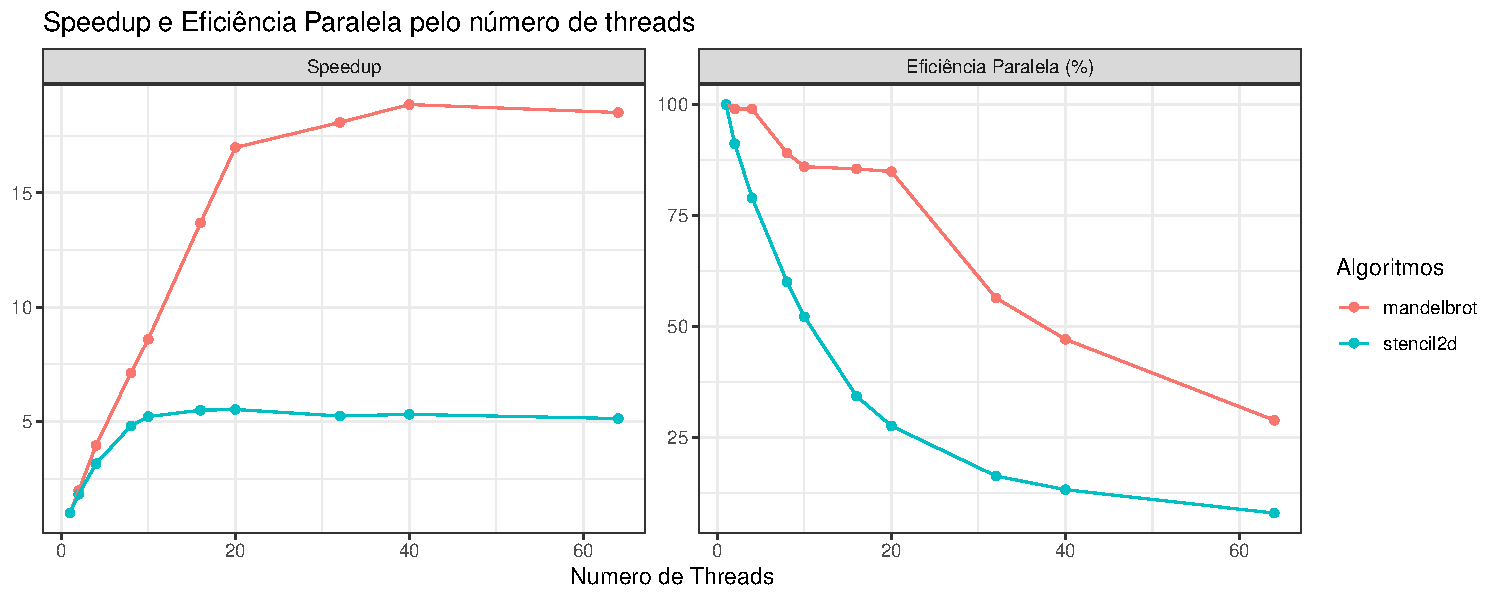
\includegraphics[width=1\textwidth]{../plots/speedup_eff.pdf}
% 	\caption{A nice plot.}
% 	\label{fig:phase1}
% \end{figure}


% \begin{figure}[h]
% 	\centering
% 	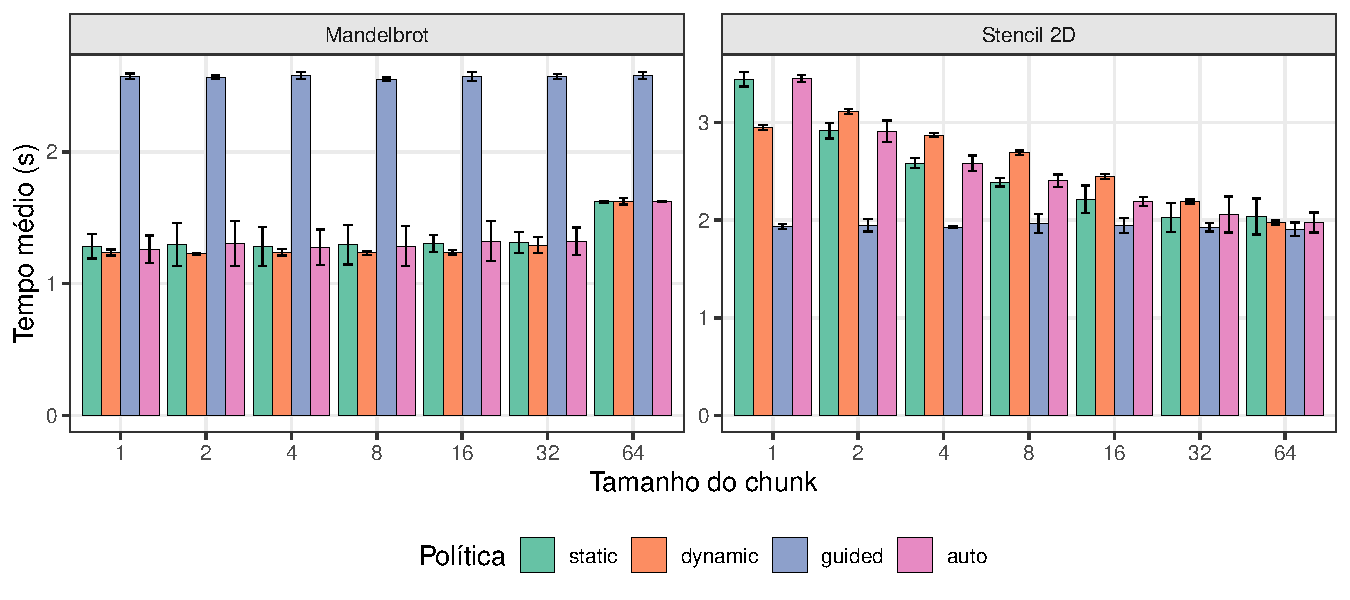
\includegraphics[width=1\textwidth]{../plots/schedule.pdf}
% 	\caption{A nice plot.}
% 	\label{fig:phase2}
% \end{figure}

% \begin{figure}[h]
% 	\centering
% 	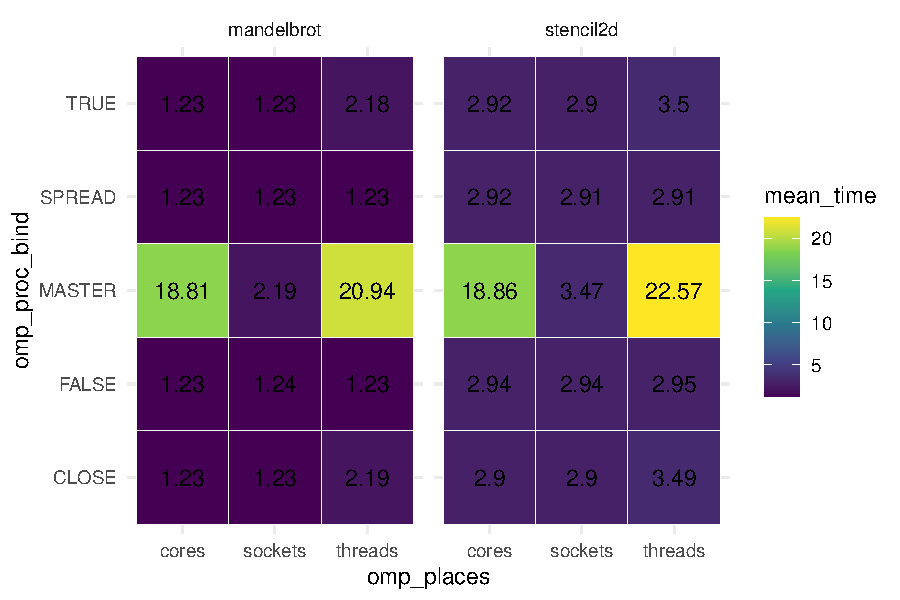
\includegraphics[width=.75\textwidth]{../plots/bind_and_places.pdf}
% 	\caption{A nice plot.}
% 	\label{fig:phase3}
% \end{figure}

% \begin{figure}[h]
% 	\centering
% 	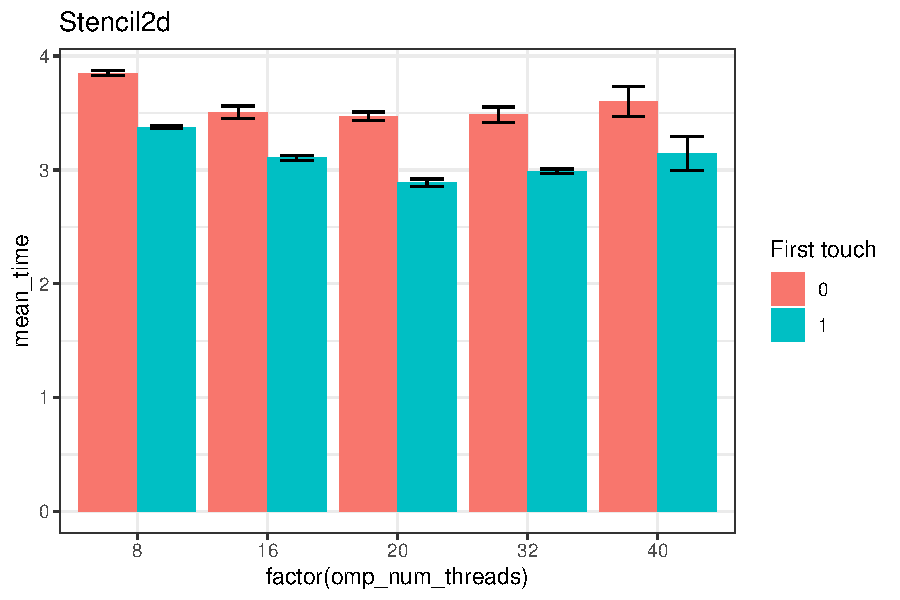
\includegraphics[width=.75\textwidth]{../plots/first_touch.pdf}
% 	\caption{A nice plot.}
% 	\label{fig:phase4}
% \end{figure}

\section{Conclusões}
% 7. Conclusões — melhores configs por app; lições obtidas na analise dos resultados.

\bibliographystyle{plain}
\bibliography{refs}

\end{document}
